%ju 31-Dez-22 09-Common-Rail-Diesel-II.tex
\section{Bauteile und Aufgaben eines Common-Rail
Systems}\label{bauteile-und-aufgaben-eines-common-rail-systems}

\begin{figure}[!ht]% hier: !ht
\centering
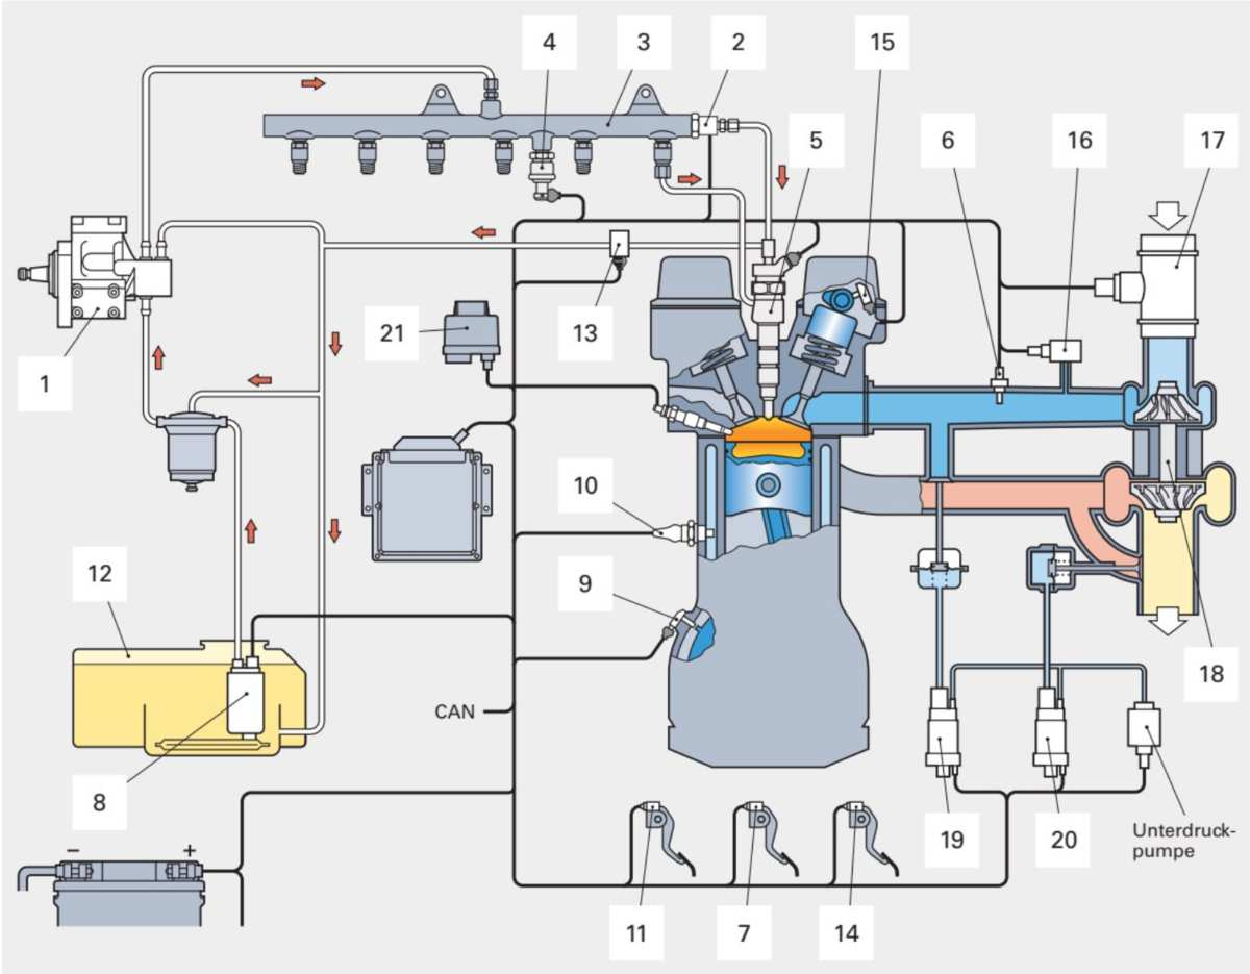
\includegraphics[width=0.7\textwidth]{images/Diesel/Diesel-6.pdf}
\caption{Common-Rail System, Quelle: Europa-Verlag}
%\label{fig:}%% anpassen
\end{figure}

\begin{enumerate}
\item
  \textbf{Hochdruckpumpe} Kraftstoff unter Hochdruck in das Rail
  fördern.
\item
  \textbf{Raildruckregelventil} den erforderlichen Hochdruck an jeden
  Betriebszustand anpassen.
\item
  \textbf{Rail} Hochdruck speichern und Verteilung des Kraftstoffs auf
  die Injektoren.
\item
  \textbf{Raildrucksensor} Hochdruck erfassen und als elektrisches
  Signal an das Steuergerät weiterleiten.
\item
  \textbf{Injektor} Kraftstoff dosiert in den Brennraum spritzen
\item
  Saugrohrtemperaturfühler
\item
  Bremspedalschalter
\item
  \textbf{Vorförderpumpe,} Kraftstoff zu Hochdruckpumpe fördern.
\end{enumerate}

\textbf{Laufruheregelung}, die einzelnen Zylinder bekommen mehr oder
weniger Kraftstoff vom Steuergerät zugeteilt.

\section{Welche Ursachen kommen für den Leistungsverlust
infrage?}\label{welche-ursachen-kommen-fuer-den-leistungsverlust-infrage}

\begin{enumerate}
\item
  \textbf{Mechanische Fehler}

  \begin{itemize}
  \item
    Kompressionsverlust durch Verschleiß der Ventile oder Kolben
  \item
    Verschleiß der Hochdruckpumpe
  \end{itemize}
\item
  \textbf{Fehler im hydraulischen System}

  \begin{itemize}
  \item
    Undichtigkeit an Injektoren (schließt nicht korrekt, tropft nach,
    Düse ausgewaschen)
  \item
    Undichte Leitungen am Rail
  \end{itemize}
\item
  \textbf{Elektrische Fehler}

  \begin{itemize}
  \item
    Sensoren defekt
  \item
    Aktoren defekt
  \item
    Leitungsunterbrechung
  \item
    Masseschluss
  \end{itemize}
\end{enumerate}

\section{Was muss beachtet werden beim Einbau eines neuen
Injektors?}\label{was-muss-beachtet-werden-beim-einbau-eines-neuen-injektors}

\begin{itemize}
\item
  Fertigungstoleranz: muss im Steuergerät einprogrammiert werden
\item
  Zahlen- und Buchstabencodes auf dem Injektor
\item
  Steuergerät korrigiert entsprechend die Grundeinspritzmenge des
  jeweiligen Injektors.
\end{itemize}

\newpage

\section{Welche Druckregelungsarten gibt es?
(Prüfung)}\label{welche-druckregelungsarten-gibt-es-pruefung}

\begin{figure}[!ht]% hier: !ht
\centering
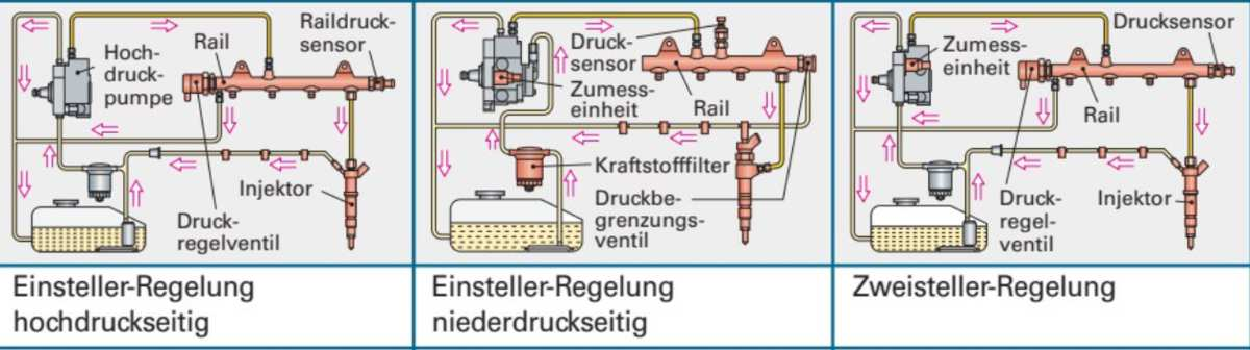
\includegraphics[width=0.8\textwidth]{images/Diesel/Diesel-2.pdf}
\caption{CR-Einsteller- und Zweistellerregelung, Quelle: Europa-Verlag}
%\label{fig:}%% anpassen
\end{figure}

\begin{enumerate}
\item
  \textbf{Einsteller-Regelung}

  \begin{itemize}
  \item
    \textbf{Druckregelung hochdruckseitig} über ein
    \textbf{Druckregelventil} (DRV)

    \begin{itemize}
    \item
      Hochdruckpumpe fördert die maximale Fördermenge unabhängig von
      Bedarf an Kraftstoff
    \item
      Raildruck wird über ein \textbf{Druckregelventil} geregelt, nicht
      benötigter Kraftstoff fließt zurück in den Tank
    \item
      \textbf{Vorteil}

      \begin{itemize}
      \item
        schneller Druckaufbau möglich
      \item
        bei Lastwechsel agil
      \end{itemize}
    \item
      \textbf{Nachteil:} Hochdruckpumpe ist konstant maximal belastet,
      dadurch

      \begin{itemize}
      \item
        geringere Nutzleistung
      \item
        erhöhter Kraftstoffverbrauch, Schadstoffausstoß, Verschleiß
      \item
        unnötige Erwärmung des Kraftstoffs
      \end{itemize}
    \end{itemize}
  \item
    \textbf{Druckregelung niederdruckseitig} (Mengenregelung) über eine
    \textbf{Zumesseinheit} (ZME)

    \begin{itemize}
    \item
      \textbf{Zumesseinheit} regelt die Zuflussmenge zur Hochdruckpumpe
    \item
      \textbf{Bedarfsregelung}, d.h. es gelangt nur so viel Kraftstoff
      zu Hochdruckpumpe wie für die Einspritzung benötigt wird
    \item
      \textbf{Druckbegrenzungsventil} verhindert zu hohen Raildruck bei
      Ausfall der Zumesseinheit
    \item
      \textbf{Vorteil}

      \begin{itemize}
      \item
        bedarfsgerechte Förderung
      \item
        geringe Leistungsaufnahme der Pumpe
      \end{itemize}
    \item
      \textbf{Nachteil:}

      \begin{itemize}
      \item
        hohe Trägheit
      \item
        Drucksteigerung erfordert zunächst eine Erhöhung des
        Niederdrucks, dadurch erhöhte Förderleistung der Hochdruckpumpe
      \end{itemize}
    \end{itemize}
  \end{itemize}
\item
  \textbf{Zweisteller - Regelung} (\textbf{Druckregelung nieder- und
  hochdruckseitig})

  \begin{itemize}
  \item
    Zusammenspiel von Zumesseinheit (ZME) und Druckregelventil (DRV)
  \item
    \textbf{Vorteile}

    \begin{itemize}
    \item
      geringe Leistungsaufnahme der Hochdruckpumpe bei konstant hohen
      Drücken
    \item
      hohe Agilität bei geringen Drücken
    \end{itemize}
  \item
    \textbf{Kaltstart / Motorstart und Warmlaufphase} (angesteuert:
    \textbf{DRV}) >>Druckregelung hochdruckseitig geregelt<<

    \begin{itemize}
    \item
      Schneller Druckaufbau möglich. Bessere Kraftstoffvorwärmung.
      Verzicht auf Kraftstoffheizung möglich.
    \item
      Kraftstoff soll sich erwärmen, um ihn damit fließ- und zündfähiger
      zu machen
    \end{itemize}
  \item
    \textbf{betriebswarmer Motor: Leerlauf / Teilllast / Schub}
    (angesteuert: \textbf{DRV und ZME}) >>Zweisteller-Betrieb<<

    \begin{itemize}
    \item
      große Sprünge des Raildrucks sind wahrscheinlich (zwischen Motor
      im Leerlauf / Teillast und $\to$ Lastwunsch des Fahrers bei
      Volllast)
    \item
      Raildruckregelung bei reduzierter Leistungsaufnahme der Pumpe
    \end{itemize}
  \item
    \textbf{hohen Motorlast} (angesteuert: \textbf{ZME}) >>Druckregelung
    niederdruckseitig geregelt<<

    \begin{itemize}
    \item
      große Steigerungen des Raildrucks nicht möglich und deshalb ist
      die Trägheit vernachlässigbar
    \item
      Reduzierter Leistungsaufnahme der Pumpe. Gesamte Kraftstoffmenge
      der Pumpe wird eingespritzt.
    \end{itemize}
  \end{itemize}
\end{enumerate}

\newpage

\textbf{Schaltstellung der Zumesseinheit an der Hochdruckpumpe in Bezug
auf die Fördermenge.}

\begin{figure}[!ht]% hier: !ht
\centering
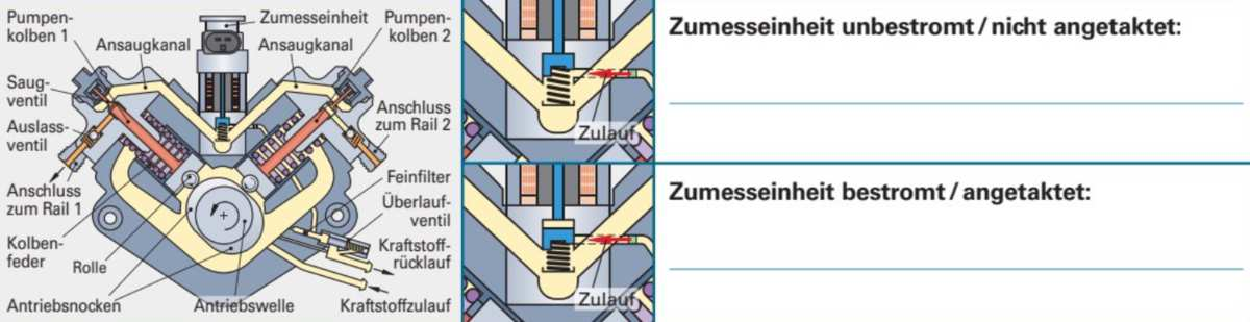
\includegraphics[width=0.8\textwidth]{images/Diesel/Diesel-3.pdf}
\caption{CR-Zumesseinheit, Quelle: Europa-Verlag}
%\label{fig:}%% anpassen
\end{figure}

\begin{enumerate}
\item
  \textbf{Zumesseinheit unbestromt}: Maximale Fördermenge
\item
  \textbf{Zumesseinheit bestromt}: verringert den Öffnungsquerschnitt
  für minimale Fördermenge
\end{enumerate}

\textbf{Druckregelventil} Druckerfassung durch Membransensor am Rail
(Raildrucksensor)

\begin{figure}[!ht]% hier: !ht
\centering
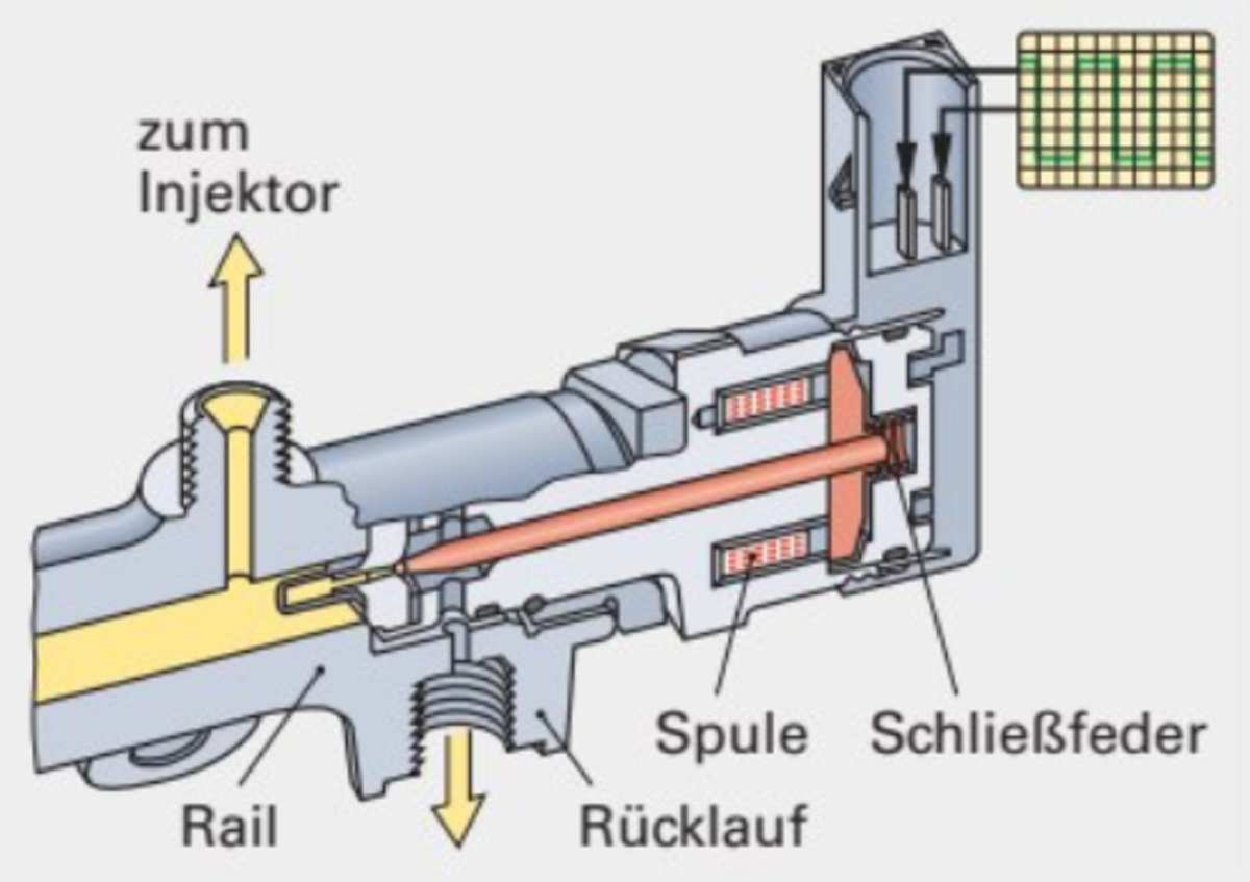
\includegraphics[width=0.3\textwidth]{images/Diesel/Diesel-8.pdf}
\caption{CR-Druckregelventil (DRV), Quelle: Europa-Verlag}
%\label{fig:}%% anpassen
\end{figure}

\emph{Ansteuerung:} Das Steuergerät taktet das Druckregelventil mit
einem PWM-Signal an. Dadurch wird die Schließkraft der Ventilnadel
erhöht oder gesenkt. Dementsprechend wird der Raildruck erhöht oder
gesenkt.

\begin{enumerate}
\item
  \textbf{Magnetventil unbestromt / stromlos} Raildruck etwa
  $100~\text{bar}$

  \begin{itemize}
  \item
    Motor abstellen, Ventilfeder hält Druckregelventil geschlossen,
    verhindert ein Leerlaufen des Rails
  \end{itemize}
\item
  \textbf{Magnetventil bestromt} Raildruck bei verschiedene
  Lastzuständen:

  \begin{itemize}
  \item
    \textbf{Motorstart} Raildruck $> 250~\text{bar}$ (Wie hoch ist der
    Druck im Rail bei Motorstart?)
  \item
    \textbf{Leerlauf} Raildruck etwa $400~\text{bar}$
  \item
    \textbf{Volllast} Raildruck etwa $2000~\text{bar}$
  \end{itemize}
\end{enumerate}

\newpage

\textbf{Warum lässt sich ein Fahrzeug mit defektem Druckregelventil
nicht mehr starten?}

\begin{figure}[!ht]% hier: !ht
\centering
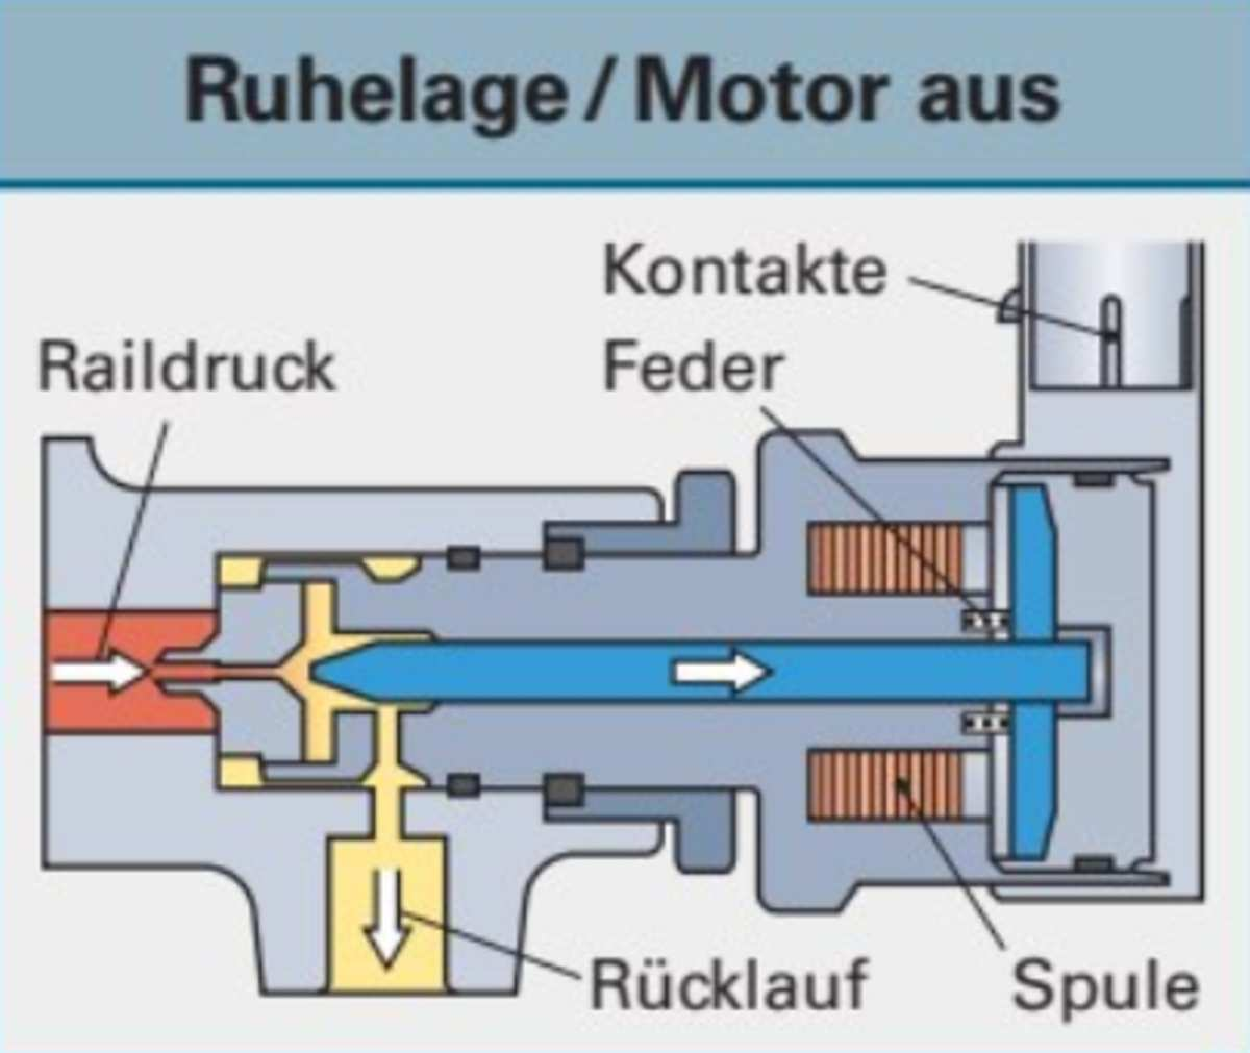
\includegraphics[width=0.3\textwidth]{images/Diesel/Diesel-4.pdf}
\caption{CR-DRV Motor aus, Quelle: Europa-Verlag}
%\label{fig:}%% anpassen
\end{figure}

Durch die im Druckregelventil verbaute Feder verbleibt im Rail ein
\textbf{Restdruck} von ca. 100 bar. Da für einen \textbf{sicheren
Motorstart} der Druck im Rail mind. 250 bar betragen muss, ist ein
Motorstart nicht möglich.

Ist die \textbf{ZME} defekt, übernimmt das \textbf{DRV} die
Druckregelung.

\newpage

\section{Injektoren}\label{injektoren}

\textbf{Unterschied zwischen Injektoren und Einspritzdüsen} haben keinen
festen Öffnungsdruck, sondern öffnen und schließen unter dem jeweiligen
variablen Einspritzdruck.

Kraft = Druck x Fläche

\subsection{Erklären Sie die Funktionsweise eines Magnetventil-Injektor
im geschlossenen und geöffneten
Zustand.}\label{erklaeren-sie-die-funktionsweise-eines-magnetventil-injektor-im-geschlossenen-und-geoeffneten-zustand.}

\begin{figure}[!ht]% hier: !ht
\centering
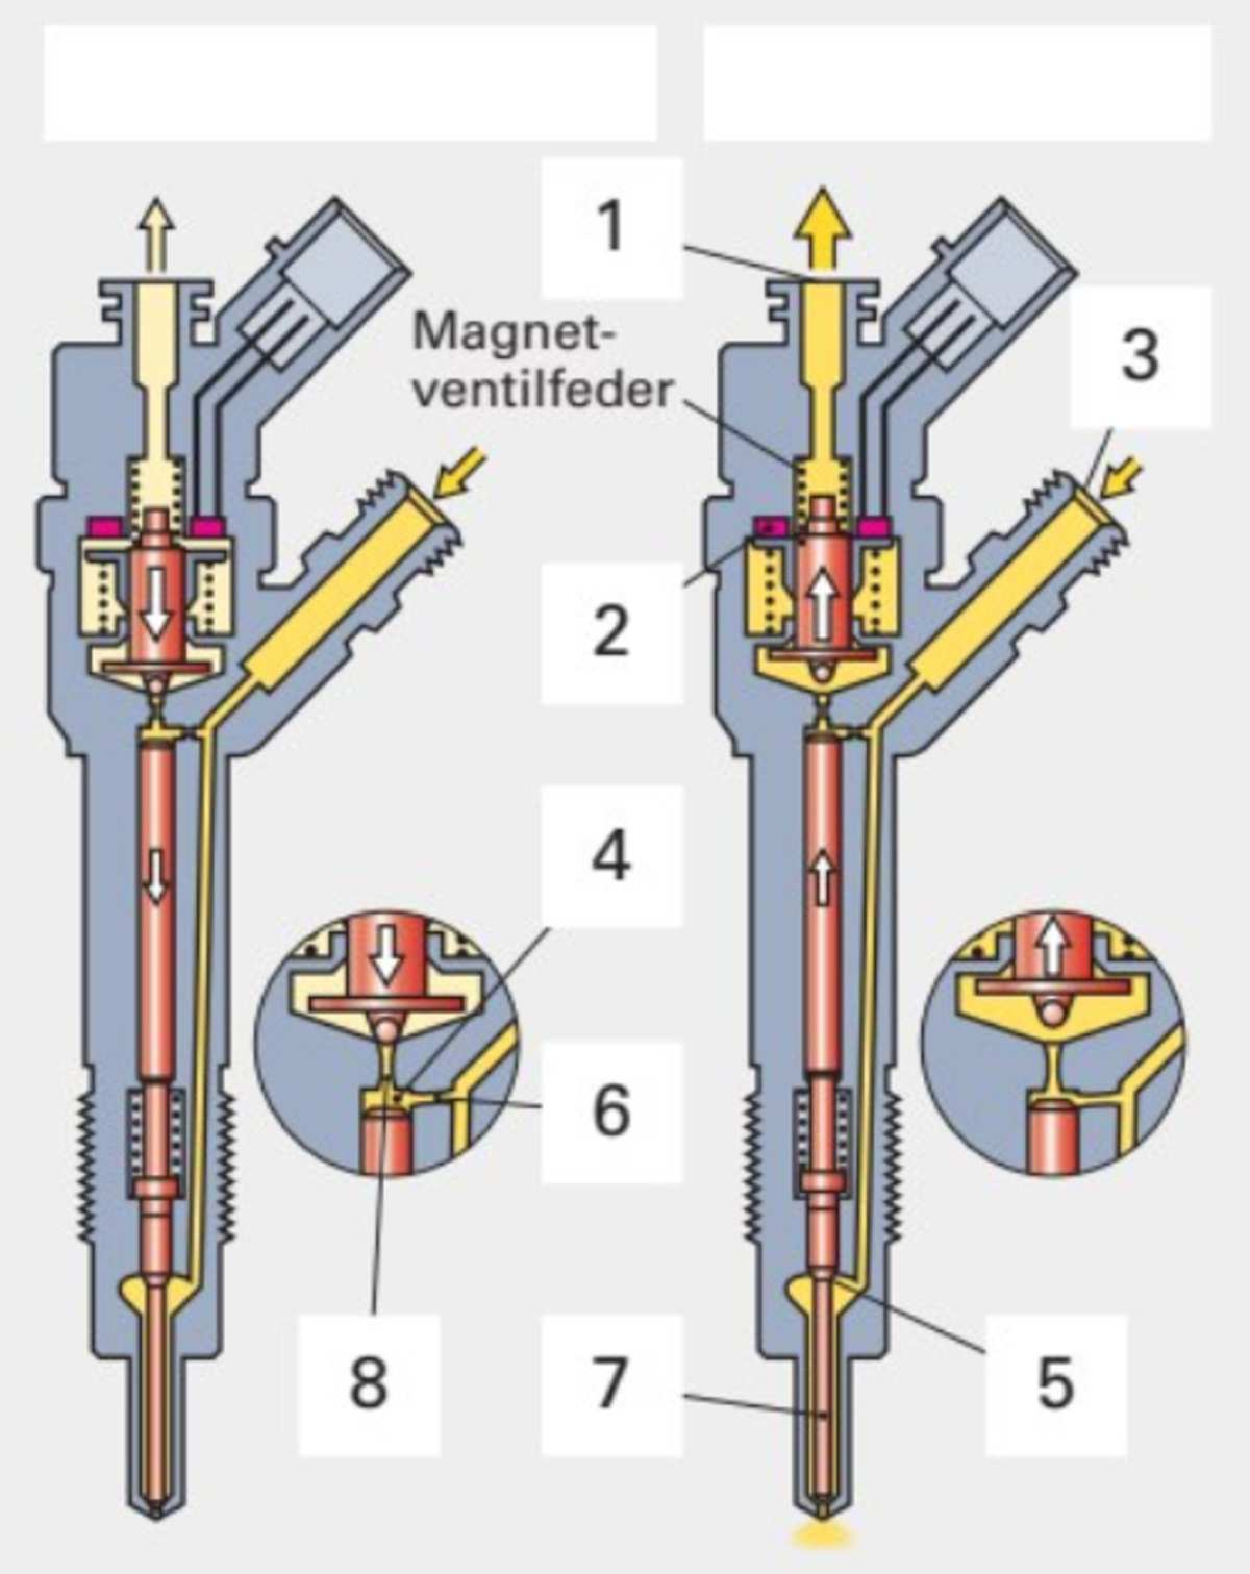
\includegraphics[width=0.3\textwidth]{images/Diesel/Diesel-7.pdf}
\caption{CR-Magnetventil-Injektor, Quelle: Europa-Verlag}
%\label{fig:}%% anpassen
\end{figure}

\begin{enumerate}
\item
  Rücklauf
\item
  Magnetventil
\item
  Zulauf von dem Rail
\item
  Ventilsteuerraum
\item
  Druckschulter
\item
  Zulaufdrossel
\item
  Düsennadel
\item
  Abflussdrossel
\end{enumerate}

\begin{itemize}
\item
  \textbf{Magnetventil unbestromt - geschlossenen Zustand} dann wirkt im
  Ventilsteuerraum auf der Stirnfläche des Ventilsteuerkolbens und auf
  der Druckschulter der Düsennadel gleicher Kraftstoffdruck.
  Einspritzventil ist geschlossen.
\item
  \textbf{Magnetventil bestromt - geöffneten Zustand,} dann wird der
  Rücklauf geöffnet. Über die Ablaufdrossel entweicht mehr Kraftstoff,
  als über die Zulaufdrossel abfließen kann. Es kommt zum Druckabfall im
  Ventilsteuerraum. Der Druck auf die Druckschulter der Düsennadel
  öffnet die Düse.
\end{itemize}

\textbf{Ansteuerung eines Magnetventil-Injektors (Spannungs- und
Stromverlauf)}

Die Injektorspannung / Boosterspannung beträgt in der Anzugsphase ca.
100 V. Der Anzugsstrom liegt dadurch bei ca. 20 A. Danach wird der Strom
auf ca. 13 A begrenzt (Haltestrom), bei einer Spannung von 12 -- 14 V
(Batteriespannung).

\textbf{Wie entsteht die Injektorspannung / Boosterspannung bis ca. 100
V?}

Beim Ausschalten der Magnetventile wird die entstehende
Selbstinduktionsspannung genutzt, um im Steuergerät einen Kondensator
aufzuladen.

\newpage

\subsection{Erklären Sie die Funktionsweise eines
Piezoinjektor}\label{erklaeren-sie-die-funktionsweise-eines-piezoinjektor}

Piezoinjektoren erlauben hohe Schaltgeschwindigkeiten und damit viele
Teileinspritzungen.

\begin{figure}[!ht]% hier: !ht
\centering
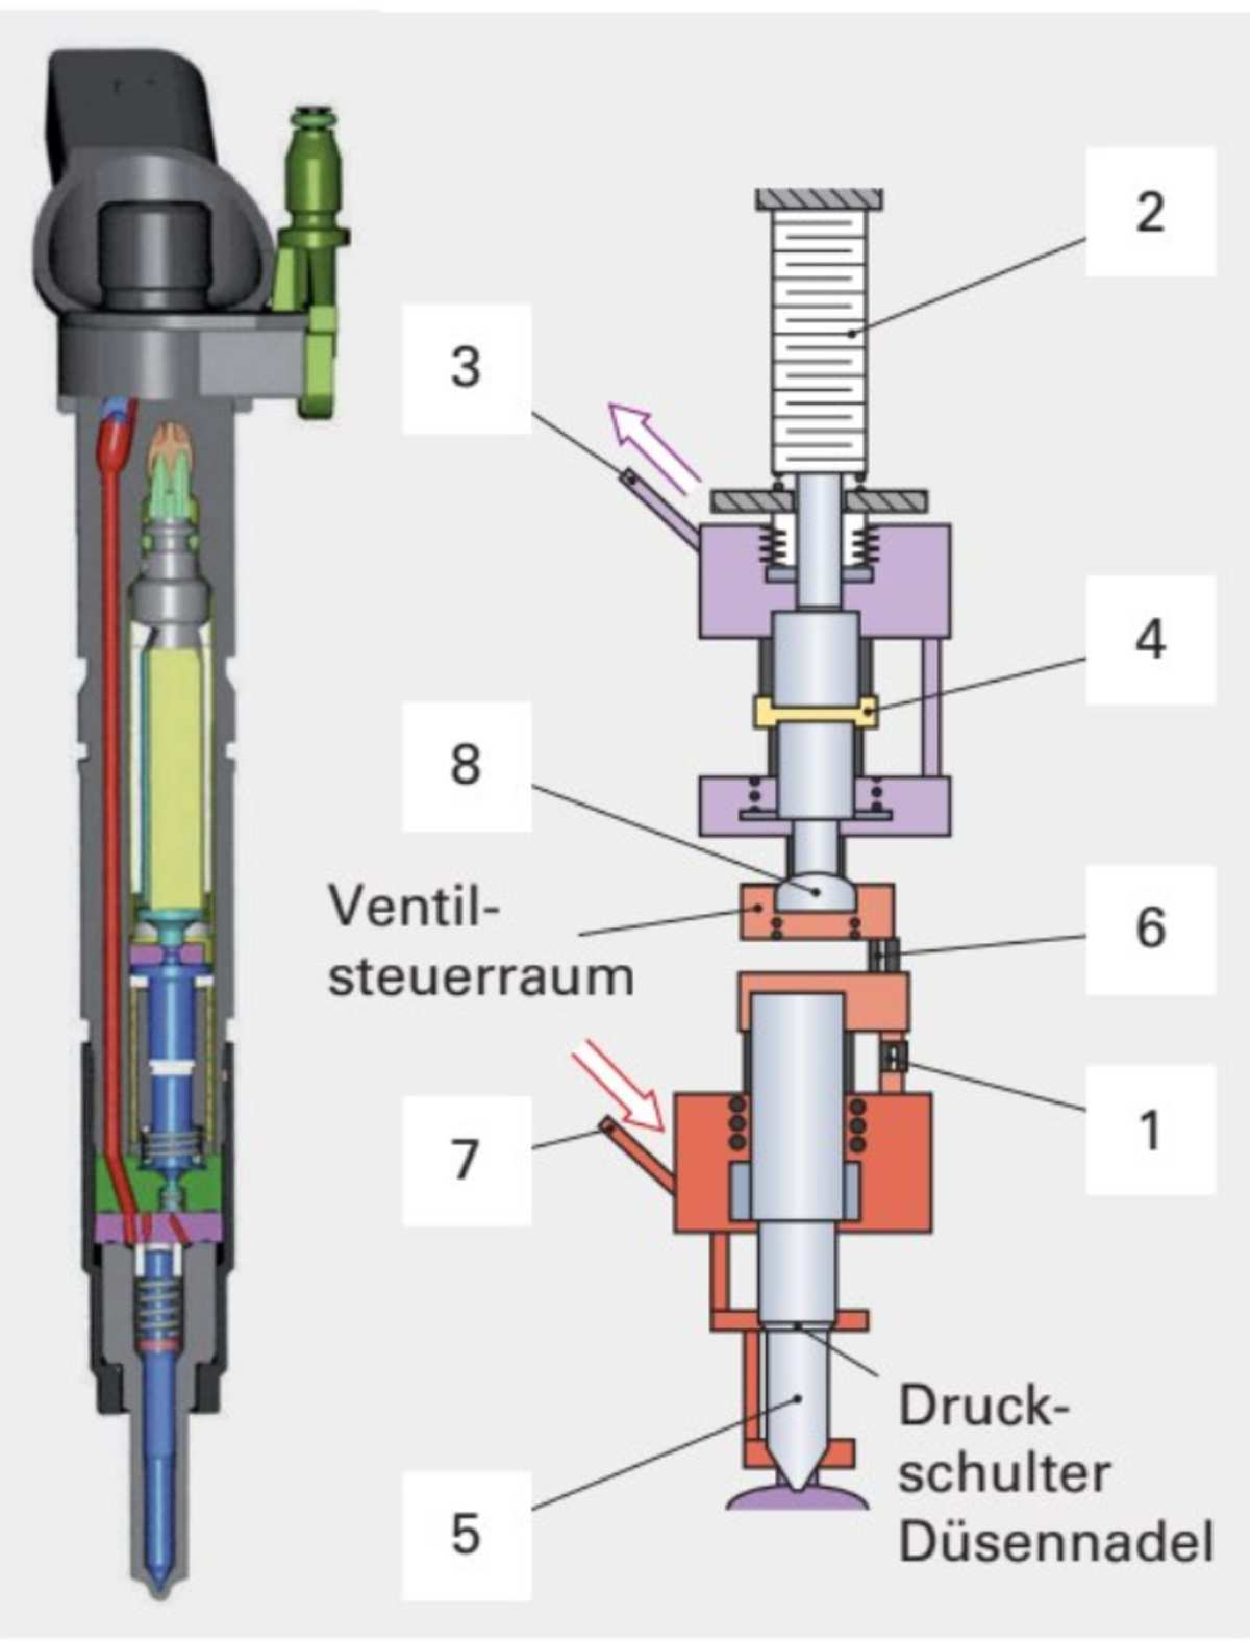
\includegraphics[width=0.3\textwidth]{images/Diesel/Diesel-1.pdf}
\caption{CR-Piezoinjektor, Quelle: Europa-Verlag}
%\label{fig:}%% anpassen
\end{figure}

\begin{enumerate}
\item
  Zulaufdrossel
\item
  Piezo-Aktormodul
\item
  Rücklauf
\item
  Hydraulischer Koppler
\item
  Düsennadel
\item
  Ablaufdrossel
\item
  Zulauf mit Raildruck
\item
  Servoventil
\end{enumerate}

\textbf{Einspritzvorgang}

\begin{enumerate}
\item
  Piezo-Aktormodul wird bestromt und dehnt sich aus
\item
  Über den hydraulischen Koppler findet eine Hubvergrößerung statt.
\item
  Der hydraulischen Koppler öffnet das Servoventil und damit den
  Rücklauf.
\item
  Über die Ablaufdrossel fließt Kraftstoff aus dem Ventilsteuerraum ab.
\item
  Über die Zulaufdrossel kann weniger Kraftstoff in den Ventilsteuerraum
  zufließen. Es kommt zum Druckabfall.
\item
  Der Druck auf die Druckschulter der Düsennadel öffnet die Düsennadel
  des Injektors. Einspritzbeginn.
\end{enumerate}

\textbf{Hydraulische Koppler vergrößert den Weg des Piezo-Aktormoduls
auf das Servoventil}

\begin{figure}[!ht]% hier: !ht
\centering
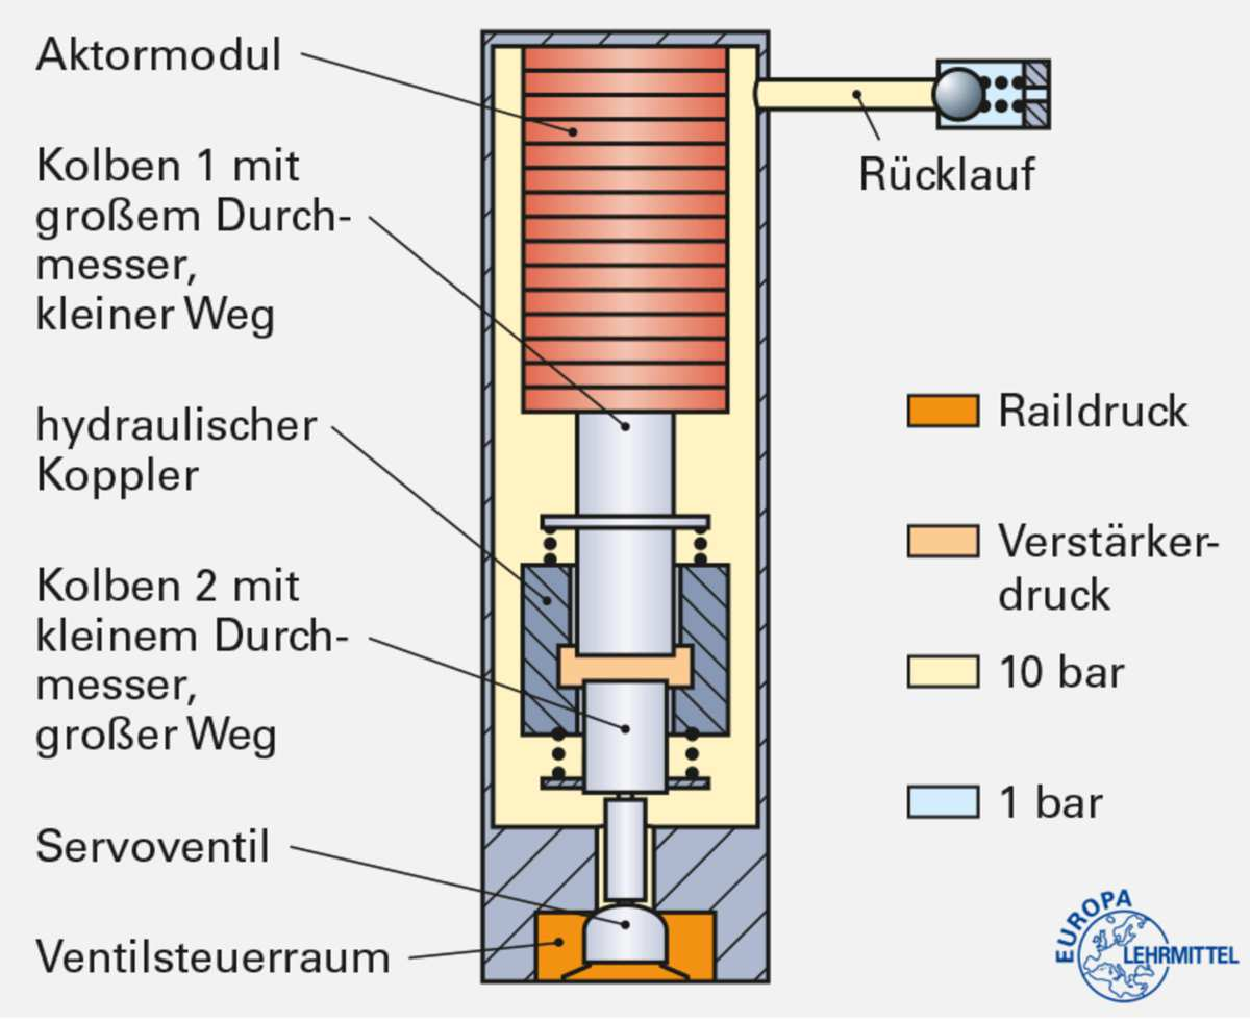
\includegraphics[width=0.3\textwidth]{images/Diesel/Diesel-21.pdf}
\caption{CR-Piezoinjektor - hydraulicher Koppler, Quelle: Europa-Verlag}
%\label{fig:}%% anpassen
\end{figure}

Er besteht aus zwei Kolben mit unterschiedlichen Durchmessern. Das
Piezo-Aktormodul drückt mit kleinem Hub auf den großen Kolben, dadurch
wird der kleine Kolben mit einem großen Hub bewegt.

\textbf{Reziproker Piezoelektrischer-Effekt} (invers) legt man an einen
Piezokristall eine Spannung an, so verformt er sich. Die Längenänderung
ist proportional zur angelegten Spannung. Bleibt in Position bis
Kurzschluss.

\emph{Verformung} durch Spannungseinfluss

\emph{Anwendung:} Injektor

\textbf{Ansteuerung eines Piezoinjektors} 110 -- 150 V bei ca. 13 A,
Piezoaktormodul dehnt sich aus (am Ende vergleichbar mit geladenen
Kondensator) \emph{Injektor offen:} Stromaufnahme null \emph{Injektor
geschlossen:} SG schaltet Spannung ab und schließt Stromkreis über
Widerstand kurz. Piezoaktormodul entlädt sich und zieht sich zusammen.

Piezoventil ersetzt Magnetventil (Grund: durch Trägheit $\to$
Magnetventil bewegt sich zeitversetzt, weil der Magnetfeldaufbau gehemmt
wird, durch Gegeninduktion)

\textbf{Piezoventil (Piezoaktor)} besteht aus Piezoaktormodul und
Übersetzermodul (kl. Hebelwerk)

Die Längenausdehnung eines Piezokristalls liegt bei maximal 0,15 \%
(sehr gering). Werden, bis zu 500 Piezokristalle in Reihe geschaltet ist
die Gesamtausdehnung des Piezoaktormodul etwa 0,04 mm. Zum Erreichen der
erforderlichen Ventilöffnung von 0,1 mm wird ein kleines Hebelwerk,
sogenannte Übersetzermodul zwischen Piezoaktormodul und hydraulischen
Ventil geschaltet.
